\documentclass{article}

\usepackage{pgf}
\usepackage{tikz}
\usetikzlibrary{arrows,automata}
\usepackage[latin1]{inputenc}
\begin{document}
	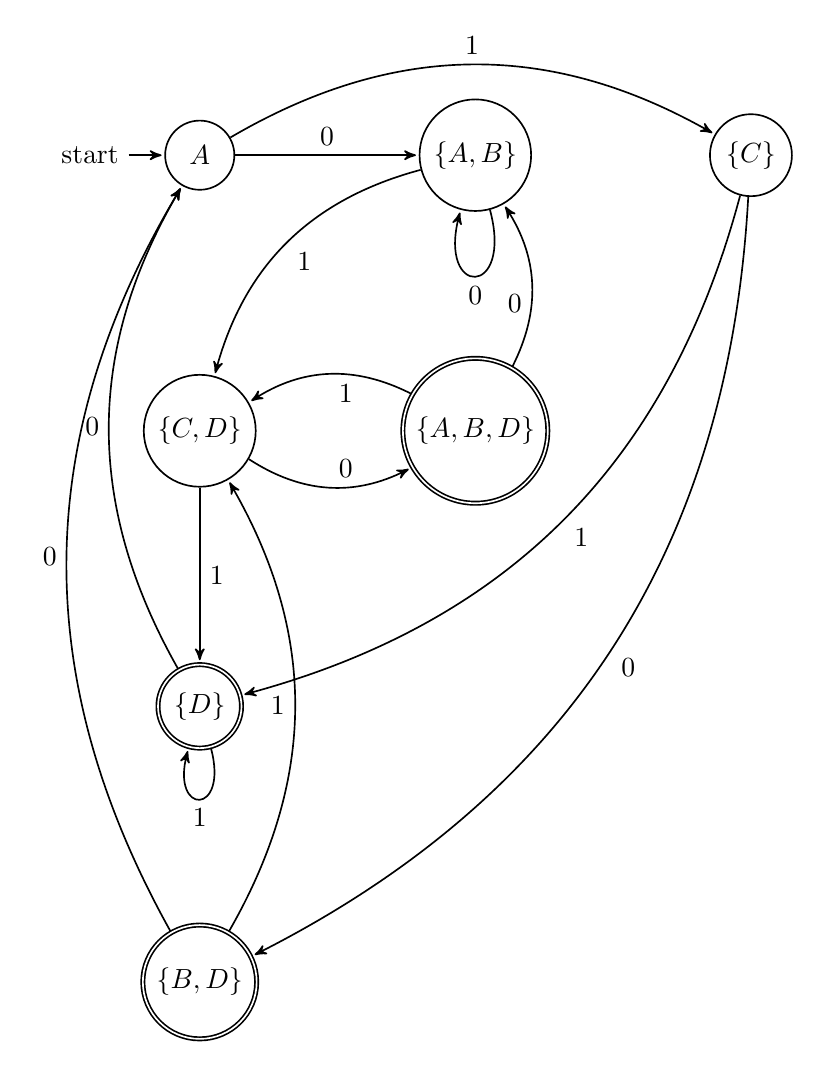
\begin{tikzpicture}[->,>=stealth',shorten >=1pt,auto,node distance=3.5cm,
	semithick]
	\tikzstyle{every state}=[fill=none,draw=#1,text=black]
	
	\node[initial,state]               (A)                    {$A$};
	\node[state]                        (B) [right of=A] {$\{A,B\}$};
	\node[state]                        (C) [right of=B] {$\{C\}$};
	\node[state,accepting]        (D) [below of=B] {$\{A,B, D\}$};
	\node[state]						(E) [below of=A] {$\{C, D\}$};
	\node[state,accepting]    	  (G) [below of=E] {$\{D\}$};
	\node[state,accepting]		  (F) [below of=G] {$\{B, D\}$};
		
	\path 
	(A) edge                       node  {0} (B)
	      edge [bend left]      node  {1}  (C)
	(B) edge [loop below]    node {0} (B)
	     edge [bend right]       node {1}  (E)
	(C) 
	     edge [bend left] node {0} (F)
	     edge [bend left]   node {1} (G)
	(D) edge [bend right]   node {1} (E)
	      edge [bend right]   node {0} (B)
	
	(E) edge [bend right]   node {0} (D)
	     edge                       node {1}  (G)
	(F) edge [bend left]   node {0} (A)
	     edge [bend right] node {1}  (E)
	(G) edge [loop below]  node {1} (G)
	      edge [bend left] node {0} (A);
	
	\end{tikzpicture}
	
\end{document}